\documentclass{beamer}
\usetheme{metropolis}
\usepackage{graphicx}
\usepackage{subfig}
\usepackage{hyperref}
\title{Algebra-Based Physics-1: Mechanics (PHYS135A-01): Unit 2}
\date{\today}
\author{Jordan Hanson}
\institute{Whittier College Department of Physics and Astronomy}

\begin{document}
\maketitle

\section{Week 3 Summary}

\begin{frame}{Week 3 Summary}
\begin{enumerate}
\item Working with vectors: displacement, velocity and acceleration
\begin{itemize}
\item Breaking into components, graphical methods
\item Analytical methods
\item \textbf{Lab-activity: testing component independence}
\end{itemize}
\item Combining free-fall and vector components: \alert{projectile motion}
\item PheT Activity: projectile motion simulation
\end{enumerate}
\end{frame}

\section{Introduction, motivation.}

\begin{frame}{Introduction to 2D kinematics}
Dude perfect basketball shots:
\url{https://youtu.be/gm2_6DX_0Bw}
\end{frame}

\section{Working with vectors: displacement, velocity and acceleration}

\begin{frame}{Working with vectors: displacement, velocity and acceleration}
In general, the displacement of an object depends on time:
\begin{equation}
\vec{r}(t) = x(t) \hat{i} + y(t) \hat{j} + z(t) \hat{k}
\end{equation}
\begin{itemize}
\item $x(t)$ is the displacement in the x-direction
\item $y(t)$ is the displacement in the y-direction
\item $z(t)$ is the displacement in the z-direction
\end{itemize}
\end{frame}

\begin{frame}{Working with vectors: displacement, velocity and acceleration}
\begin{figure}
\centering
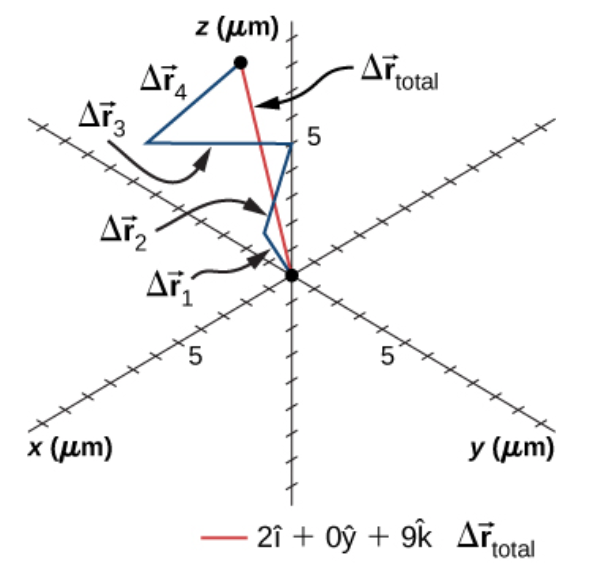
\includegraphics[width=0.6\textwidth,trim=0cm 2cm 0cm 0cm,clip=true]{figures/Brownian.png}
\caption{\label{fig:brown} An example of a displacement vector at different moments in time.}
\end{figure}
\end{frame}

\begin{frame}{Working with vectors: displacement, velocity and acceleration}
The particle in Fig. \ref{fig:brown} has four displacement vectors at four moments in time:
\begin{itemize}
\item $\vec{r}_{\rm 1} = 2.0\hat{i} + 1.0\hat{j} + 3.0\hat{k}\quad(\mu m)$ at $t_{\rm 1}$
\item $\vec{r}_{\rm 2} = -1.0\hat{i} + 0.0\hat{j} + 3.0\hat{k}\quad(\mu m)$ at $t_{\rm 2}$
\item $\vec{r}_{\rm 3} = 4.0\hat{i} + -2.0\hat{j} + 1.0\hat{k}\quad(\mu m)$ at $t_{\rm 3}$
\item $\vec{r}_{\rm 4} = -3.0\hat{i} + 1.0\hat{j} + 2.0\hat{k}\quad(\mu m)$ at $t_{\rm 4}$
\end{itemize}
What is the total displacement of the particle from the origin?
\end{frame}

\begin{frame}{Working with vectors: displacement, velocity and acceleration}
We can think of this type of problem as an accounting problem, lining up columns (units: $\mu m$):
\begin{figure}
\begin{tabular}{| c | c | c | c | c |}
\hline
$t_{\rm i}$ & $\vec{r}_{\rm i}(t_{\rm i})$ & $x(t_{\rm i})$ & $y(t_{\rm i})$ & $y(t_{\rm i})$ \\
\hline
$t_{\rm 1}$ & $\vec{r}_{\rm 1}(t_{\rm 1})$ & 2.0 & 1.0 & 3.0 \\
\hline
$t_{\rm 2}$ & $\vec{r}_{\rm 2}(t_{\rm 2})$ & -1.0 & 0.0 & 3.0 \\
\hline
$t_{\rm 3}$ & $\vec{r}_{\rm 3}(t_{\rm 3})$ & 4.0 & -2.0 & 1.0 \\
\hline
$t_{\rm 4}$ & $\vec{r}_{\rm 4}(t_{\rm 4})$ & -3.0 & 1.0 & 2.0 \\
\hline
\hline
$t_{\rm total}$ & $\vec{r}_{\rm total}(t_{\rm total})$ & 2.0 & 0.0 & 9.0 \\
\hline
\end{tabular}
\caption{\label{tab:account} Accounting for the different displacement components, in units of $\mu m$.}
\end{figure}
\end{frame}

\begin{frame}{Working with vectors: displacement, velocity and acceleration}
\begin{figure}
\centering
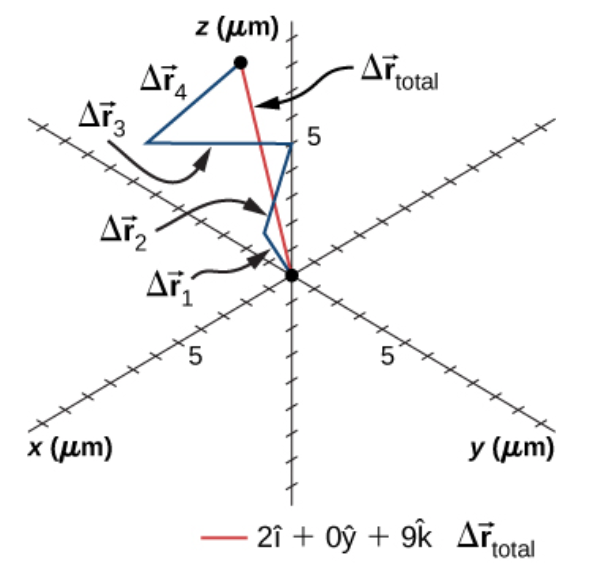
\includegraphics[width=0.4\textwidth]{figures/Brownian.png}
\caption{\label{fig:brown2} The total displacement of the particle is $\vec{r}_{\rm total} = 2.0\hat{i} + 0.0\hat{k} + 9.0\hat{k}\quad (\mu m)$.}
\end{figure}
\textbf{Professor: work several examples.}
\end{frame}

\begin{frame}{Working with vectors: displacement, velocity and acceleration}
\small
The 18th hole at Pebble Beach Golf Course is a dogleg to the left of length 496.0 meters.  The fairway off the tee is taken to be the x direction.  A golfer hits his tee shot a distance of 300 meters, corresponding to a displacement of $\vec{r}_{\rm 1} = 300.0 \hat{i} \quad (m)$, and then hits a second shot 189.0 meters with $\vec{r}_{\rm 2} = 150.0 \hat{i} + 80.0 \hat{j} \quad m$.  What is the final displacement from the tee?
\begin{itemize}
\item A: $\vec{r}_{\rm final} = 150.0 \hat{i} + 80.0\hat{j}\quad (m)$
\item B: $\vec{r}_{\rm final} = 450.0 \hat{i} + 230.0\hat{j}\quad (m)$
\item C: $\vec{r}_{\rm final} = 230.0 \hat{i} + 0.0\hat{j}\quad (m)$
\item D: $\vec{r}_{\rm final} = 450.0 \hat{i} + 80.0\hat{j}\quad (m)$
\end{itemize}
\end{frame}

\begin{frame}{Working with vectors: displacement, velocity and acceleration}
\small
If the first shot takes 5.0 seconds, the second shot takes 4.0 seconds, and the walking time in between the shots is 60.0 seconds, what is the average velocity vector for the ball after the two shots?
\begin{itemize}
\item A: $\vec{r}_{\rm final} = 50.7 \hat{i} + 11.6\hat{j}\quad (m/s)$
\item B: $\vec{v}_{\rm final} = 17.0 \hat{i} + 80.3\hat{j}\quad (m/s)$
\item C: $\vec{v}_{\rm final} = 6.5 \hat{i} + 1.2\hat{j}\quad (m)$
\item D: $\vec{v}_{\rm final} = 6.5 \hat{i} + 1.2\hat{j}\quad (m/s)$
\end{itemize}
\end{frame}

\begin{frame}{Working with vectors: displacement, velocity and acceleration}
The prior problem indicates something you may already have guessed:
\begin{equation}
\vec{v}_{\rm avg}(t) = v_{\rm x}(t) \hat{i} + v_{\rm y}(t) \hat{j} + v_{\rm z}(t) \hat{k} = \frac{\Delta\vec{r}}{\Delta t}
\label{eq:vel}
\end{equation}
\begin{itemize}
\item $v_{\rm x}(t)$ is the avg. velocity in the x-direction
\item $v_{\rm y}(t)$ is the avg. velocity in the y-direction
\item $v_{\rm z}(t)$ is the avg. velocity in the z-direction
\end{itemize}
In other words, we divide each displacement component by the time, to get a vector where each component is the average velocity in that direction.  $\Delta\vec{r} = \vec{r}_{\rm f} - \vec{r}_{\rm i}$.
\end{frame}

\begin{frame}{Working with vectors: displacement, velocity and acceleration}
An x-ray is radiated from a radioactive source, and travels at the speed of light (0.3 m/ns) 60 degrees with respect to the x-axis, in the positive direction.  A person's broken leg is 1.0 m to the right of the radioactive source.  When does the gamma ray reach the person?
\begin{itemize}
\item A: $20/\sqrt{3}$ ns
\item B: $20/(3\sqrt{3})$ ns
\item C: $20/3$ ns
\item D: $10$ ns
\end{itemize}
\end{frame}

\begin{frame}{Working with vectors: displacement, velocity and acceleration}
A person changes lanes on a highway.  Her vehicle is traveling at 100 km/hr.  She turns the wheel so that the car's velocity points 20 degrees from the direction down the highway.  By what percentage must she increase her speed in order to maintain 100 km/hr \textit{down the highway}?
\begin{itemize}
\item A: 1\%
\item B: 2\%
\item C: 6\%
\item D: 10\%
\end{itemize}
\end{frame}

\begin{frame}{Working with vectors: displacement, velocity and acceleration}
In the kinematic description of motion, \alert{\textit{we are able to treat the different components of motion separately.}}  In many cases, motion in the horizontal direction does not affect motion in the vertical direction, and vice versa.\\
\vspace{0.5cm}
\small
\framebox[1.1\width]{\textbf{Motions in displacement components are independent.}} \\
\vspace{1cm}
\textit{(Exception: non-conservative forces.  More on this later.)}
\end{frame}

\begin{frame}{Projectile motion}
\small
\begin{figure}
\centering
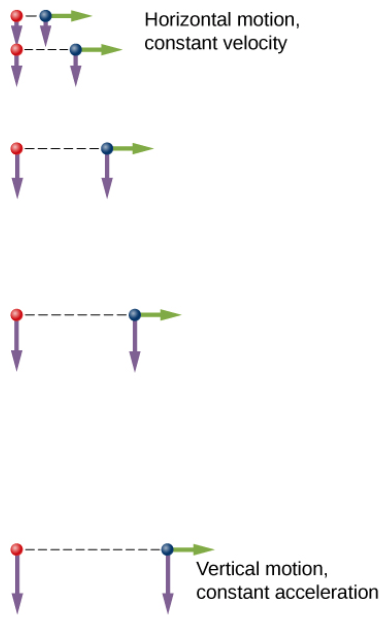
\includegraphics[width=0.4\textwidth]{figures/fall.png}
\caption{\label{fig:fall} Independence of motion in two dimensions.}
\end{figure}
\end{frame}

\begin{frame}{Projectile motion}
Is this true?  Figure \ref{fig:fall} is testable by experiment. \\
\vspace{0.5cm}
\small
Procedure:
\begin{enumerate}
\item Obtain two marbles, a meter stick, and a stopwatch.
\item Measure the height of the lab bench, $\Delta x$.
\item We are going to drop a marble from this height ($\Delta x$) and record the time.  Show first algebraically that the predicted time for the marble to fall is $t = \sqrt{2\Delta x/g}$.
\item Measure $t$ for several trials.  Does it match the expected result $\sqrt{2\Delta x/g}$?  What are sources of error?
\item Repeat the measurement, but \textbf{roll the marble off of the table at varying speed}.  Does the average result for $t$ change?
\end{enumerate}
\end{frame}

\section{Combining free-fall and vector components: projectile motion}

\begin{frame}{Projectile motion}
\small
We now have learned that (a) motions in displacement components are \textit{independent}, and (b) when acceleration is in \alert{one direction} (vertical) only, the motion is \textit{projectile motion}.  Our usual equations of motion for no acceleration (horizontal), and constant acceleration (vertical) apply \textit{independently}:
\begin{columns}[T]
\begin{column}{0.5\textwidth}
\begin{align}
y(t) &= y_{\rm 0} + v_{\rm 0,y} t - \frac{1}{2}gt^2 \label{eq:main1} \\
v_{\rm y}(t) &= -gt+v_{\rm 0,y} \label{eq:main2} \\
v_{\rm y}^2 &= v_{\rm y,0}^2 - 2g(y-y_{\rm 0}) \label{eq:main3}
\end{align}
\end{column}
\begin{column}{0.5\textwidth}
\begin{align}
x(t) &= x_{\rm 0} + v_{\rm 0,x}t \label{eq:main4} \\
v_{\rm x}(t) &= v_{\rm 0,x} \label{eq:main5}
\end{align}
\end{column}
\end{columns}
\end{frame}

\begin{frame}{Projectile Motion}
\small
Projectile motion is a good topic to introduce the concept of \textit{boundary conditions}.  The \textit{physics} of projectile motion is the same for all situations, but the \textit{individual cases and numbers} might not be the same. \\
\vspace{0.5cm}
Suppose we are given the initial velocity and angle of a object that undergoes projectile motion.  To use Eqs. \ref{eq:main1}-\ref{eq:main5}, we need $v_{\rm 0,x}$ and $v_{\rm 0,y}$, the initial horizontal and vertical velocity components, respectively.
\end{frame}

\begin{frame}{Projectile Motion}
\small
Suppose we are given the initial velocity and angle of a object that undergoes projectile motion.  To use Eqs. \ref{eq:main1}-\ref{eq:main5}, we need $v_{\rm 0,x}$ and $v_{\rm 0,y}$, the initial horizontal and vertical velocity components, respectively.\\
\begin{figure}
\centering
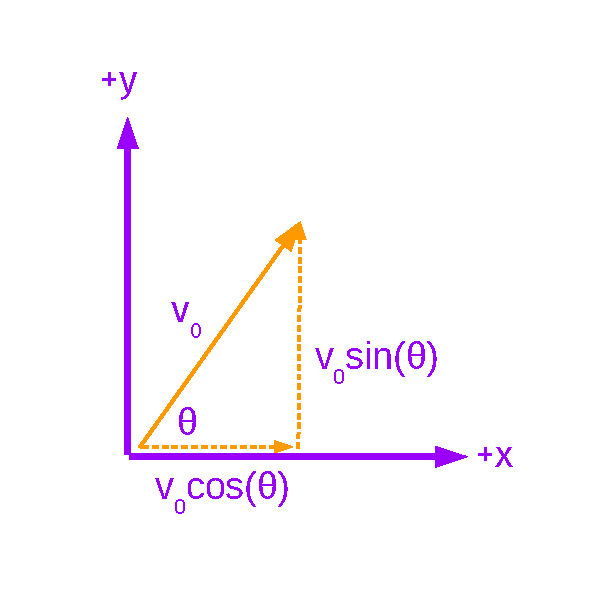
\includegraphics[width=0.5\textwidth,trim=1cm 1cm 1cm 1cm,clip=true]{figures/Vectors1.pdf}
\caption{\label{fig:components} The initial velocity $v_{\rm 0}$ is broken into components.}
\end{figure}
\end{frame}

\begin{frame}{Projectile Motion}
\small
\textbf{Professor: set this one up with a diagram, work two examples first.} \\
During a fireworks display, a shell is shot into the air with an initial speed of 50 m/s, at an angle of 60$^{\circ}$ above horizontal.  The fuse is timed to ignite the shell just as it reaches its highest point above the ground.  Calculate the height at which the shell explodes.
\begin{itemize}
\item A: 190 m
\item B: 100 m
\item C: 110 m
\item D: 250 m
\end{itemize}
\end{frame}

\begin{frame}{Projectile Motion}
\small
How much time passes between the launch and the explosion?
\begin{itemize}
\item A: 3.9 seconds
\item B: 4.3 seconds
\item C: 5.1 seconds
\item D: 10.0 seconds
\end{itemize}
\end{frame}

\begin{frame}{Projectile Motion}
What is the horizontal displacement of the shell when it explodes?
\begin{itemize}
\item A: 108 meters
\item B: 98 meters
\item C: 98 degrees
\item D: 150 meters
\end{itemize}
\end{frame}

\section{PhET Activity}

\begin{frame}{Projectile Motion}
\small
Let's try gaining visual intuition about projectile motion through the following program: \\
\vspace{0.25cm}
\url{https://phet.colorado.edu/en/simulation/projectile-motion}\\
\begin{enumerate}
\item Derive the \textit{range equation} (Professor on board).
\item Plot the range versus initial velocity, for some fixed $\theta$.  Use Excel to derive the relationship by fitting a trend line to the data.
\item Plot the range versus $\theta$, for some fixed initial velocity.  Use Excel to derive the relationship by fitting a trend line to the data.
\item Now, turn on air resistance, and repeat the prior two exercises.  What do you notice about the trend lines?
\item Play with the air resistance parameter by tuning it with the tools on the right side of the screen.  What do you notice?
\end{enumerate}
\end{frame}

\begin{frame}{Projectile Motion}
Projectile motion in two dimensions, with constant acceleration in one dimension, produces \textit{quadratic curves}.  How do we obtain the \alert{trajectory}, or $y(x)$ for these curves?  Looking at the x-direction:\\
\begin{align}
x &= v_{\rm 0}\cos(\theta) t \\
t &= \frac{x}{v_{\rm 0} \cos(\theta)} \label{eq:subst}
\end{align}
\end{frame}

\begin{frame}{Projectile Motion}
Substituting in Eq. \ref{eq:subst} for $t$ into the equation for vertical displacement gives:\\
\begin{align}
y(t) - y_{\rm 0} &= -\frac{1}{2}g\frac{x^2}{v_{\rm 0}^2\cos^2(\theta)} + \tan(\theta) x \\
y(t) - y_{\rm 0} &= -\left(\frac{g}{2v_{\rm 0}^2\cos^2(\theta)}\right)x^2 + \tan(\theta) x \\
y(x) &= -kx^2 + bx + y_{\rm 0}\label{eq:projfinal}
\end{align}
In Eq. \ref{eq:projfinal}, we are simply saying that $y(x)$ is some quadratic.  (It's still true that $y$ and $x$ are both functions of \textit{time}, however, those functions of time are related).
\end{frame}

\begin{frame}{Projectile Motion}
A space explorer is on a moon around another planet, and wants to measure $g$.  She tosses a pebble from an initial height of 2 meter, at an angle of 45 degrees above horizontal, with an initial velocity of 2 m/s.  When it lands, the horizontal displacement is 10 meters.  What is the gravitational acceleration $g$?
\begin{itemize}
\item A: 0.125 m/s$^2$
\item B: 0.25 m/s$^2$
\item C: 0.5 m/s$^2$
\item D: 1.0 m/s$^2$
\end{itemize}
\end{frame}

\begin{frame}{Projectile Motion}
Other useful equations are for the \textit{time-of-flight}, and the \textit{range}, concepts we've already seen in several examples: \\
\begin{align}
T_{\rm tof} &= \frac{2v_{\rm 0}\sin\theta}{g} \\
R &= \frac{v_{\rm 0}^2\sin2\theta}{g}
\end{align}
\end{frame}

\section{Conclusion}

\begin{frame}{Week 3 Summary}
\begin{enumerate}
\item Working with vectors: displacement, velocity and acceleration
\begin{itemize}
\item Breaking into components, graphical methods
\item Analytical methods
\item \textbf{Lab-activity: testing component independence}
\end{itemize}
\item Combining free-fall and vector components: \alert{projectile motion}
\item PheT Activity: projectile motion simulation
\end{enumerate}
\end{frame}

\end{document}
